\documentclass{school-22.211-notes}
\date{April  2, 2012}

\begin{document}
\maketitle

\lecture{Numerical Solutions for Diffusion Theory}
\topic{Simple Numerical Methods to Solve Diffusion Equations}
\subtopic{Derivation of Neutron Balance Equation}
Recall the two-group neutron balance equations:
\begin{itemize}
\item Total fission source is: 
  \eqn{S_f(r) = \mu \Sigma_{f1} (r) \phi_1 (r) + \mu \Sigma_{f2} (r) \phi_2(r) }
  $\xi_1 = 1, \xi_2 = 0$ which implies that fission source in the thermal group is zero.
\item Scattering source: we define effective down-scattering, so up-scattering is zero $\Sigma_{21}(r) = 0$. 
\item Two-group diffusion equations: 
\eqn{-\gradient D_1 \divergence \phi_1 + [\Sigma_{a1} + \Sigma_{s12}] \phi_1 = \nu \Sigma_{f1} \phi_1 + \nu \Sigma_{f2} \phi_2 + S_1} 
\eqn{-\gradient D_2 \divergence \phi_2 + \Sigma_{a2} \phi_2 = \Sigma_{s12} \phi_1 + S_2}
\end{itemize}

\subtopic{Derivation of Interface Flux}
Then we construct a finite spatial mesh in which cross sections are constant; integrate the neutron diffusion equations over each mesh cell $\Delta^n$,
\eqn{-\int \ddx D_1^n \ddx \phi_1^n \dx + \Sigma_{r1}^n  \phi_1^n \Delta^n = \nu \Sigma_{f1}^n \phi_1^n \Delta^n + \nu \Sigma_{f2}^n \phi_2^n \Delta^n + S_1 \Delta^n} 
\eqn{-\int \ddx D_2^n \ddx \phi_2^n  \dx + \Sigma_{a2}^n \phi_2^n \Delta^n = \Sigma_{s12}^n \phi_1^n \Delta^n + S_2 \Delta^n}
We evaluate the integral term\footnote{Lectuer says use the divergence theorem $\int \divergence \vec{F} \dV = \int_S \vec{F} \cdot \vec{n} \dS$, I think this is just manipulating integral and $\int \ddx A \dx \to A$}, 
\eqn{\int \ddx D_1^n \ddx \phi_1^n \dx  = \left. D_1^n \ddx \phi_1^n \right|_{n^+} - \left. D_1^n \ddx \phi_1^n \right|_{n^-} }
Then we have,
\eqn{\left. D_1^n \ddx \phi_1^n \right|_{n^-} - \left. D_1^n \ddx \phi_1^n \right|_{n^+} + \Sigma_{r1}^n  \phi_1^n \Delta^n = \nu \Sigma_{f1}^n \phi_1^n \Delta^n + \nu \Sigma_{f2}^n \phi_2^n \Delta^n + S_1 \Delta^n} 
\eqn{\left. D_2^n \ddx \phi_2^n \right|_{n^-} - \left. D_2^n \ddx \phi_2^n \right|_{n^+} + \Sigma_{a2}^n \phi_2^n \Delta^n = \Sigma_{s12}^n \phi_1^n \Delta^n + S_2 \Delta^n}
We notice that the $-D \ddx \phi$ terms are just flux terms (in fact, they are the interface fluxes):
\eqn{J_n^+ = - \left. D_g^n \ddx \phi_g^n \right|_{n+} = -D_g^n \frac{\phi_g^S - \phi_g^n}{\Delta/2} }
\eqn{J_n^- = - \left. D_g^{n+1} \ddx \phi_g^{n+1} \right|_{n-} = - D_g^{n+1} \frac{\phi_g^{n+1} - \phi_g^s}{\Delta/2} }
By continuity of the net current, we can set the above two equations to equal to each other, 
\eqn{  -D_g^n \frac{\phi_g^S - \phi_g^n}{\Delta/2} =  - D_g^{n+1} \frac{\phi_g^{n+1} - \phi_g^s}{\Delta/2} }
From where we can solve for the interface flux, 
\eqn{ \phi_g^s = \frac{D_g^{n+1} \phi_g^{n+1} + D_g^n \phi_g^n}{D_g^n + D_g^{n+1}}} 
Then we can get th net current in terms of mesh fluxes: 
\eqn{ J_n^+ = - \frac{2D_g^n}{\Delta} \left[ \frac{ D^{n+1} \phi^{n+1} + D^n \phi^n}{D^n + D^{n+1}} - \phi^n \right] = - \overbrace{\frac{2 D^n D^{n+1} }{\Delta (D^n + D^{n+1})}}^{\to \hat{D}^{n,n+1}} (\phi^{n+1} - \phi^{n}) }
That is, 
\eqn{J_n^+ &= - \hat{D}^{n,n+1} (\phi^{n+1} - \phi^n)  & J_n^- &= - \hat{D}^{n-1, n} (\phi^n - \phi^{n-1} ) \label{net-current}}


\subtopic{Derivation of Finite Difference Equations}
Plug Eq.~\ref{net-current} back into diffusion equations, we get, 
\eqn{ \hat{D}_1^{n-1,n} (\phi_1^n - \phi_1^{n-1})  - \hat{D}_1^{n,n+1} (\phi_1^{n+1} - \phi_1^n) + \Sigma_{r1}^n \phi_1^n \Delta^n &= \mu \Sigma_{f1}^n \phi_1^n \Delta^n + \mu \Sigma_{f2}^n \phi_2^n \Delta^n + S_1 \Delta^n} 
\eqn{ \hat{D}_2^{n-1,n} (\phi_2^n - \phi_2^{n-1})  - \hat{D}_2^{n,n+1} (\phi_2^{n+1} - \phi_2^n) + \Sigma_{a2}^n \phi_2^n \Delta^n &= \Sigma_{s12}^n \phi_1^n \Delta^n + S_2 \Delta^n} 
Rearranging terms by fluxes, we get, 
\eqn{ - \hat{D}_1^{n-1,n} \phi_1^{n-1} - \hat{D}_1^{n,n+1} \phi_1^{n+1} + [ \Sigma_{r1}^n \Delta^n + \hat{D}_1^{n-1, n} + \hat{D}_1^{n,n+1} ] \phi_1^n = \nu \Sigma_{f1}^n \phi_1^n \Delta^n + \nu \Sigma_{f2}^n \phi_2^n \Delta^n + S_1^n \Delta^n} 
\eqn{ - \hat{D}_2^{n-1,n} \phi_2^{n-1} - \hat{D}_2^{n,n+1} \phi_2^{n+1} + [\Sigma_{a2}^n \Delta^n + \hat{D}_2^{n-1.n} + \hat{D}_2^{n,n+1} ] \phi_2^n = \Sigma_{s12}^n \phi_1^n \Delta^n + S_2^n \Delta^n }

\subtopic{Derivation of Boundary Condition}
Interior of the geometry, the boundary conditions are implied. The exterior boundaries have to be specified. There are two types of boundary conditions:
\begin{enumerate}
\item Zero Flux BC: 
\eqn{ J_g^N = -D_g^N \frac{ -\phi_g^N - \phi_g^N}{\Delta^N}  = \frac{2 D_g^N}{\Delta^N} \phi_g^N }
\item Zero Incoming Current BC:
\eqn{ J^- = \frac{1}{4} \phi - \frac{1}{2} J_n = 0 }
which implies,
\begin{align}
  J_g^N &= \frac{\phi_g^s}{2} = -D_g^N \frac{\phi_g^s - \phi_g^N}{\Delta/2} \\
  &= - \frac{2 D_g^N}{\Delta^N} \frac{\frac{2D_g^N}{\Delta^N} - 1}{\frac{1}{2} + \frac{2D_g^N}{\Delta}} \phi_g^N \\
  &= \boxed{ \frac{2D_g^N}{\Delta^N} \left[ \frac{1}{1 + \frac{4 D_g^N}{\Delta^N}} \right] \phi_g^N } \label{JgN}
\end{align}
In Eqn.~\ref{JgN}, if $D \to 0$, we get zero flux boundary condition; if $D \to \infty$, we get zero current boundary condition. 
\end{enumerate}

\clearpage
\topic{Matrix Representation of 1D Slab Diffusion Equations}
\subtopic{Construct Matrix}
If we use $L$ for the $\phi^{n-1}$ term, $U$ for the $\phi^{n+1}$ term, $D$ for the $\phi^n$ term, $T$ for the transport term, we can express the finite difference equation in matrix form as: 
\begin{align}
[L_1 + D_1 + U_1] [\phi_1] &= [M_1] [\phi_1] + [M_2][\phi_2] + [S_1] \\
[L_2 + D_2 + U_2] [\phi_2] &= [T_2] [\phi_1] + [S_2] 
\end{align}
We define a vector of group fluxes, 
\begin{align}
\left[ \begin{array}{cc} 
[L_1 + D_1 + U_1] & [0] \\
-[T_2] & [L_2 + D_2 + U_2] \\
\end{array} \right] 
\left[ \begin{array}{c}
\phi_1 \\ \phi_2 \\ \end{array} \right] 
= \left[ {\begin{array}{cc} \left[M_1\right] & \left[M_2\right] \\ \left[0\right] & \left[0\right] \end{array}} \right] 
\left[ \begin{array}{c}
\phi_1 \\ \phi_2 \\ \end{array} \right] 
+ 
\left[ \begin{array}{c} 
S_1 \\ S_2 \\ \end{array} \right] 
\end{align}
Whose compressed form is, 
\eqn{ [A] [\phi] = [M] [\phi] + [S] }
The two matrix are plotted in Figure~\ref{matrix-form}. Notice there are missing points in A; explaination: Block matrix: there is no coupling of group 1 left flux to the group 2 right flux. 
\begin{figure}
  \centering
  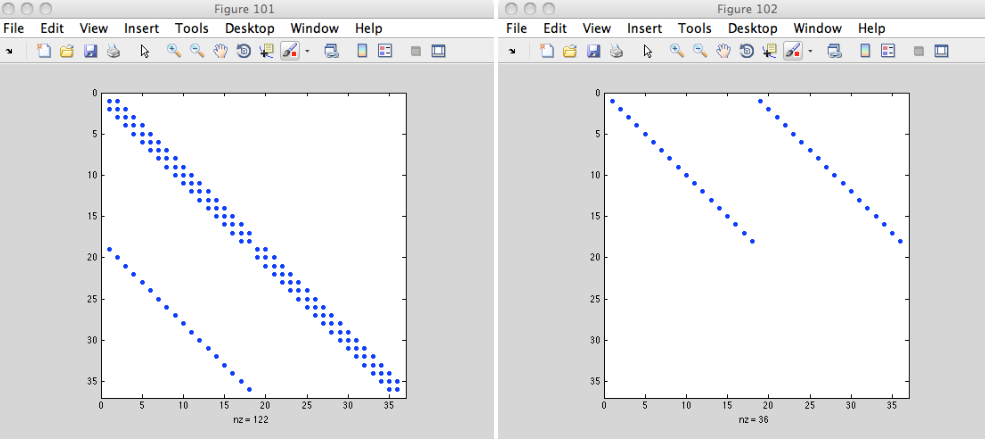
\includegraphics[width=4in]{images/dfs/matrix-form.png}
  \caption{Destruction and Production Matrix} \label{matrix-form}
\end{figure}


\subtopic{Method 1: Sequential Source/Fixed-Source Problem}
\begin{align}
[A] [\phi] &= [M] [\phi] + [S] \\
[A - M ] [\phi] &= [S] \\
[\phi] &= [A - M]^{-1} [S]
\end{align}
In this method, we guess $\keff$, and given a source we can solve for the flux. We never solve real questions this way, because 

If we have a super-critical problem, then the only way to get criticality with an additional source is through negative flux. 

A reactor is like an amplifier; the closer it is to criticality the more amplification it is; when critical, the amplification is infinity. 


\subtopic{Method 2: Direct Matlab Eigenvalue Solver}
We can solve for $\keff$ directly from: 
\begin{align}
[A] [\phi] &= \frac{1}{\keff} [M] [\phi] \\
[A]^{-1} [M] [\phi] &= \keff [\phi]
\end{align}
Notice that the eigenvectors are arbitrarily normalized; hence it is fine if the flux is negative. 


\subtopic{Method 3: Power Iterations}
\begin{align}
[A] [\phi]^{n+1} &= [M] [\phi]^n \\
\keff &= \frac{[M][\phi]^{n+1} }{[M] [\phi]^n} 
\end{align}
The rate our fission source converges depends on material, geometry etc. \hi{The dominance ratio} is defined as $\frac{\lambda_1}{\lambda_2}$; and it is 0.97 for this example. If we know the dominance ratio of the problem, we can estimate the number of iterations needed to converge. 
\begin{figure}
  \centering
  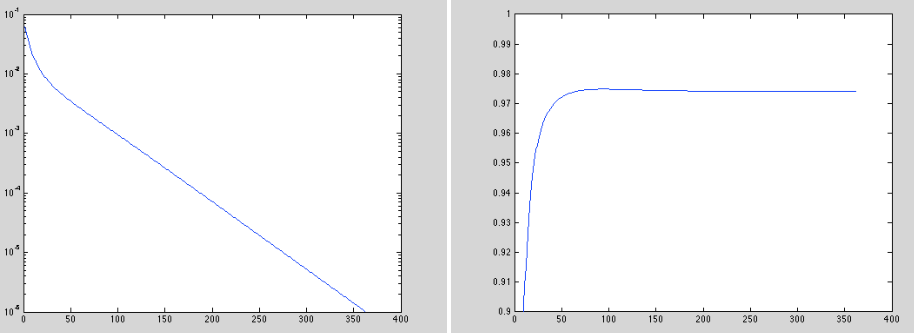
\includegraphics[width=4in]{images/dfs/power-iteration-convergence.png}
  \caption{The Convergence Rate of Power Iteration}
\end{figure}

\subtopic{Method 3+: Power Iterations with Gauss-Jacobi Numerical Inversion of Flux Matrix}
See Lec. 12 slide 21. In a steady-state problem, it does not matter whether we fully converge our flux iteration. 


\clearpage
\topic{Matrix Representation of Higher Dimensions Diffusion Equations}
Insert image from p.14 Lec13. 

\begin{enumerate}
\item 1D matrix can be solved without iterations, but not for higher dimenisions. We have to use iterative methods for higher dimensions. 
\item The matrix representation looks the same as in 1D, except with one additional pair of off-diagonal term for each additional dimension. 
\item The size of the matrix goes up. For instance, if we have 10 meshes per dimension, then 1D matrix is 10x10, 2D matrix is 100x100, 3D matrix is 1000x1000.
\end{enumerate}


\clearpage
\topic{Dominance Ratio}
The relationship between dominance ratio and convergence ratio: convergence rate = 1 - dominance ratio in most numerical methods. 
\begin{enumerate}
\item Symmetric mode. If initial guess is symmetric, solution is symmetric, and the method used is symmetric, then only the symmetric mode shows up in the dominance ratio, and the asymmetric mode is hidden. In our case  [FIXME]

\item Core size: 

\item Decoupling of radial zone. For instance, if we insert control rod, or have asymmetric core loadings, or have xenon distributions,  the radial zones decoupled, dominance ratio decreases. 

\item Decoupling of axial zones form partially inserted control rods, axial fuel enrichment zoning, axial burnable absorber loading. 
\end{enumerate}
Dominance ratio measures the spatial decoupling. 

\topic{HW5: Numerical Solution of Solving Two-Group Diffusion Problems}
It is not just iterative convergence that we care; spatial convergence is required as well. Core design: reflector, fuel 1, fuel 2, fuel 1, reflector, decide which fuel goes on the inside and where the boundaries are. 


\clearpage
\topic{Summary}
Remember for real 3D problem,
\begin{itemize}
\item Matrix inversion if of order $N^3$, so in real applications no matrix inversion;
\item Finding all eigenvalues if at least order $N^2$;
\item Iterative inversion must be order $N$ to be practical for large problems;
\item Multi-level iteration is a practical necessity. 
\end{itemize}


\end{document}
